\chapter{Privacy-preserving KYC on Ethereum}

\label{Chapter12KYC}

In this Chapter, we describe the current approach to identity management and propose KYCE -- a privacy-preserving KYC scheme for token whitelisting on Ethereum.\footnote{This Chapter is based on~\cite{Biryukov2018}, which, in turn, described a hackathon project. The team consisting of Daniel Feher, Dmitry Khovratovich, Sergei Tikhomirov, Aleksei Udovenko, and Maciej \.{Z}urad implemented a proof-of-concept implementation in May~2017 during the Luxblock hackathon in Luxembourg and won a joint first prize. Contributions of the author of this thesis include: implementing parts of the hackathon project and writing the paper (except for Section~\ref{sec:PrivacyPreservingKYC}).}


\section{Identity}

Digital identity is the information used by a computer system to represent a user.
Access to services is controlled in two steps:

\begin{itemize}
	\item authentication: a user proves that they are who they claim to be;
	\item authorization: the system ensures that the user has the right to perform the requested action.
\end{itemize}

To comply with regulations, financial institutions verify the identities of their customers.
Modern finance depends on government-issued identities.
Regulations in most jurisdictions demand that banks obtain proof of identity from customers before doing business with them -- a procedure known as "know your customer," or KYC.
"Anti money laundering" (AML) and "counter terrorist financing" (CTF) are related regulations that require banks to stop and report suspicious transactions.

Modern KYC practices weaken users' control over their personal information and threaten their privacy.
Financial institutions store sensitive information in private databases, which become a target for corrupt employees or external hackers.
Implement KYC/AML implementations lead to high compliance cost and multiplies the risk of identity theft.

Open blockchains like Ethereum take a more decentralized approach to identity management.
Users join these networks without any identification.
Financial service providers establish consortia to apply blockchain technologies in their services~\cite{EEA2017, Hyperledger, R3}.
To comply with regulation, they have to handle government-issued identities in a blockchain setting.
This non-trivial task becomes more challenging, considering users' demands for stronger privacy protection.
The European privacy regulation (GDPR~\cite{GDPR16}) that came into force in May~2018 poses more challenges for organizations that handle personal data.

In this work, we first explore the centralized and decentralized approaches to identity.
We then propose KYCE -- a privacy-preserving Ethereum-based KYC implementation.
KYCE allows banks to implement KYC checks using an external smart contract -- a KYC provider.
Our scheme uses zero-knowledge proofs to check users' eligibility without disclosing their private information to anyone except the KYC provider.
A smart contract stores the KYC whitelist in the form of a cryptographic accumulator.
This construction allows users to be efficiently added to, removed from, and checked against the list without storing any plaintext data on the blockchain.
We then discuss possible use cases and implementation challenges.

\subsection{Centralized identity}

In terms of asymmetric cryptography, identity~$I$ of user~$U$ is a public-private key pair~$(pub_U, priv_U)$.
The public key~$pub_U$ authenticates the user (or, equivalently, links the current action to some past actions).
Public identifiers like username or address are derived from~$pub_U$.
The private key~$priv_U$ allows $U$ to sign messages on behalf of~$I$.
For the system, $U$ is whoever possesses $priv_U$.

In the centralized identity model, prevalent on the Internet today, users delegate managing their private keys to a trusted party and use a password to access them when necessary.
This approach is sub-optimal in many regards.
First, users do not control their identities.
The trusted party always has the technical ability to sign messages without the user's consent or to prevent the user from signing the message they want.
Moreover, users' data is stored by a centralized entity, providing incentives for an attack.
Finally, users have to create a new identity for each website they wish to register with.
As a result, they adhere to a risky practice of reusing passwords.
Third-party login protocols such as OAuth and OpenID~\cite{Dodanduwa2018} partially address this issue ("login with").
In this scheme, a website queries the website that holds the user's existing identity (e.g.,~Google) and asks for permission to access a subset of the user's data (e.g.,~name and email).
This approach alleviates the password management problem but increases the impact of potential identity theft.

Though users can revoke access at any time, the "login with" scheme is still privacy-violating.
Imagine a user who reveals their birth date to prove to a website that they are 18 years of age or older.
If they later revoke the access, their date of birth will never change.
Thus, they grant the third-party website effectively unlimited access to a piece of private information.

Maintaining correspondence between "real world" identities and public keys has long been a challenge.
Widely deployed centralized solutions like PKI suffer from risks associated with centralization: a fraudulent authority can issue rogue certificates~\cite{Amann2017}.


\subsection{Decentralized identity and open blockchains}

The PGP "web of trust" is a noteworthy attempt at creating a decentralized identity system~\cite{Feisthammel2017}.
It has not gained significant traction due in part to usability challenges~\cite{Ruoti2015} and concerns about the security of the long-term key model~\cite{Valsorda2016}.

Bitcoin~\cite{Nakamoto2008} eliminates the problem of connecting public keys to identities in a radical manner: a user may generate many public keys that \textit{are} identities.
Alternative blockchains such as Ethereum~\cite{Buterin2014, Wood2014} take a similar approach.
The way open blockchains handle identity may come at odds with financial regulation.
We propose a design that will simultaneously leverage the power of blockchain-based smart contracts, enable banks to implement KYC to comply with the law, and preserve users' privacy.


\subsection{Financial and privacy regulation in the EU} \label{sec:Ch12KYCEU}

The current EU legislation "on information accompanying transfers of funds" came into effect in 2015~\cite{EU847}.
In the wake of the rapid growth of cryptocurrencies, the EU is tightening its anti-money laundering regulations, stating that "virtual currency exchange platforms and custodian wallet providers will have to apply customer due diligence controls, ending the anonymity associated with such exchanges"~\cite{EU16}.
See~\cite{Vandezande2017} for the analysis of virtual currencies under the EU AML law.

In 2018, two pieces of legislation came into force in the EU\@.

\begin{itemize}
	\item The \textbf{Revised Payment Service Directive} (PSD2) obligates banks to provide access to their customers' accounts through open APIs~\cite{Hellstroem2017}.
	This measure is meant to foster competition and give rise to third-party financial service providers.
	For instance, a unified banking API would simplify connecting banking infrastructure to open blockchains~\cite{Elison2016}.
	\item The \textbf{General Data Protection Regulation} (GDPR) harmonizes data privacy laws across the EU~\cite{GDPR16} and introduces stricter rules for handling data of EU residents even for companies from outside the EU\@. We refer the reader to~\cite{Berberich2016} describes possible implications of blockchain adoption from the viewpoint of the EU data protection regulation.
\end{itemize}


\section{KYCE: a decentralized KYC-compliant exchange}

KYC requirements differ depending on jurisdiction~\cite{PWC2015}.
A typical KYC procedure links users' real-world identities to their accounts and checks users against a whitelist or a blacklist.
The details of the KYC procedure do not affect our design.

\subsection{Definitions and security properties}

\begin{definition}
	A \textbf{KYC procedure} is a process that determines if a given user is eligible for a given transaction.
\end{definition}

\begin{definition}
	A \textbf{KYC provider} is an entity that performs a KYC procedure.
\end{definition}

\begin{definition}
	A \textbf{financial service} is an information system that allows users to exchange units of value.
\end{definition}

\begin{definition}
	A financial service is \textbf{KYC-compliant} w.r.t.~the KYC procedure if and only if all users are eligible for all transactions they perform.
\end{definition}

\begin{definition}
	A KYC-compliant financial service is \textbf{privacy-preserving} if and only if only the KYC provider has access to the users' private data.
\end{definition}


\subsection{Tokens and exchanges}

Our KYC solution can be applied for any service.
For concreteness, consider a token exchange as an example of an exchange.

\begin{definition}
	A \textbf{token} is a transferable fungible unit of value maintained by a smart contract.
\end{definition}

ERC20~\cite{Victor2019} is the de-facto standard API for implementing token contracts in Ethereum.
A token contract keeps track of users' token balances and enables them to transfer tokens using the following functions:

\begin{itemize}
	\item \texttt{transfer} sends a given amount of tokens to a given address;
	\item \texttt{approve} allows a given user to withdraw up to a given amount of tokens from the account of the user calling the function;
	\item \texttt{transferFrom} sends a given amount of tokens from one given address to another (the amount has to be \texttt{approve}d beforehand).
\end{itemize}

\begin{definition}
	An \textbf{exchange} is a service that enables users to exchange tokens.
\end{definition}

Centralized exchanges, implemented as a regular web service, are the most prevalent.
We are mostly interested in decentralized, or on-chain exchanges, implemented as smart contracts.

An exchange without KYC support may be used as follows.
\begin{enumerate}
	\item Alice creates an order to sell $X$~A-tokens for $Y$~B-tokens;
	\item Bob creates an order to sell $Y$~B-tokens for $X$~A-tokens;
	\item The exchange matches the two orders and transfers (by calling \texttt{transferFrom}) $X$~A-tokens from Alice to Bob and~$Y$~B-tokens from Bob to Alice.
\end{enumerate}

The transaction succeeds if Alice and Bob have \texttt{approve}d the exchange with a sufficient amount of A- and B-tokens, respectively, before \texttt{transferFrom} is called.
Users withdraw tokens from the exchange by calling \texttt{approve(exchangeAddress,0)}.



\subsection{Privacy-preserving KYC}
\label{sec:PrivacyPreservingKYC}

We propose KYCE -- a privacy-preserving KYC design for Ethereum-based financial service providers.
A KYC contract provides an API to other contracts so that external services can determine if a given user is KYC-approved for using a given token.
A KYC provider (a governmental entity or company in charge of customer onboarding) performs the necessary checks for a new customer and adds their address to the whitelist.

A simple approach to implementing a KYC check with a separate contract would be the following.
The KYC contract stores the whitelist of approved addresses.
On every \texttt{transfer}, token contracts check if the address belongs to the whitelist.
This design has a fundamental privacy flaw: the contract stores all whitelisted addresses on-chain in plaintext.
Moreover, users must use the same addresses they have registered with the KYC provider.
Address reuse threatens privacy: an adversary can link the user's transactions using public blockchain data.

\paragraph{Our approach}
We use cryptographic techniques to design a privacy-preserving KYC solution.
In KYCE, the KYC contract stores a \textbf{cryptographic accumulator} of the whitelisted addresses. 

A cryptographic accumulator~$A$ absorbs certain algebraic objects and provides an interface to generate and verify zero-knowledge proofs that a given value has been accumulated.
In our construction, to generate a proof for value~$x\in A$, one needs a \textit{witness} that depends on~$A$ and~$x$.
The accumulator owner provides the witness to the user who submitted $x$.
We suggest an accumulator based on bilinear maps~\cite{Camenisch2009}.

The KYC workflow is as follows.
The KYC provider publishes a smart contract and initializes it with an empty accumulator.
The User interacts with the KYC provider physically or online and provides the credentials needed to pass the verification.
The User also generates their own master secret~$m$ and during the authenticated session, gives the provider a Pedersen commitment~$g_1^m\cdot g_2^r$ to it.
$g_1$ and~$g_2$ are certain group generators\footnote{Here and in the further text all multiplications take place in the pre-selected group of prime order~$q$, typically an elliptic-curve group.}, and~$r$ is random.
If the User passes the procedure, the provider updates the accumulator with user-dependent data and gives the User a witness.
In every subsequent Ethereum transaction to KYCE, the User provides a proof that they have been registered in the accumulator, that this right has not been revoked, and that the proof owner and the transaction sender are one person.
KYCE verifies the last statement.
The KYC contract verifies the rest against the current accumulator value.
If the checks pass, KYCE executes the requested action.

\paragraph{Details on the accumulator construction}
We construct an accumulator based on a pairing function~$e(\cdot,\cdot)$ in some pairing setting.\footnote{The original paper~\cite{Camenisch2009} uses type-1 pairings, but type-3 pairings can be adopted as well.}.
The accumulator contains the serial numbers, possibly consecutive integers.\footnote{It is possible to store public keys, but it would be less efficient.}

The accumulator is constructed as follows.
We assume a bilinear pairing~$e:\,G\times G\rightarrow G_T$, where $G,G_T$ are groups of order~$q$.
The KYC provider selects a generator~$g$ and a secret value $\gamma\overset{\$}{\leftarrow} \mathbb{Z}_q$.
It also selects $L$ as an upper bound of users enabled for KYC and computes $z = e(g,g)^{\gamma^{L+1}}$.
It initialized the accumulator value~$\mathrm{A}$ by $1$. 

Let us denote $g_i = g^{\gamma^i}$.
The provider publishes $\mathrm{A},\{g_i\}_{1\leq i\leq L, \,L+2\leq i \leq 2L}$, the set of registered KYC indices $V=\emptyset$, and the parameters $g,z$ needed for verification.

Every User who passes the KYC check is issued a new serial number~$i$, the witness~$w_i = \prod_{j\in V,j\neq i} g_{L+1-j+i}$, where $V$ is the set of all issued serial numbers, and a signature~$\sigma_i$ of~$g_i||i$ on the provider's private signature key.
The witness is used to generate a proof of accumulating.\footnote{We refer an interested reader to~\cite{Camenisch2009} for the details.}
The KYC provider updates the accumulator with~$i$ by
$$
\mathrm{A_{V\cup\{i\}}} \leftarrow \mathrm{A_V} \cdot g_{L+1-i}
$$
multiplying it by $g_{L+1-i} = g^{\gamma^{L+1-i}}$, and~$i$ is published as a new valid serial number.
To prove that $i$ has been committed to $A$ and has not been revoked without disclosing it, the holder of~$w_i$ updates it\footnote{We omit the details, but the update can be performed just before the presentation, not necessarily after every accumulator update.} so that the following equation holds:
$$
\frac{e(g_i, A)}{e(g,w_i)} = z.
$$

Note that revocation is also efficient.
The KYC contract owner simply multiplies the accumulator value by the inverse of~$g_{L+1-i}$.
The witness value cannot be updated anymore.

\paragraph{Presentation} 
When issuing a transaction to use the exchange (e.g.,~create an order), the user submits a \textbf{zero-knowledge proof} of the following statement:
\begin{itemize}
	\item I know the private key of the current user address (\texttt{msg.sender}), and
	\item I know a signature~$\sigma_i$ and a witness~$w_i$ for some number~$i$ that has been accumulated in the
	accumulator~$A$ in the KYC contract.
\end{itemize}
This compound statement must be \textit{atomic}, i.e.,~the sub-statements cannot be extracted as separate valid proofs, as this would make the transaction malleable.

The atomicity (and non-malleability) are ensured as follows.
Let us denote the proof of knowledge for the witness and signature by~$PK_w$.
Then the Prover submits 
$$
P = \{PK_w \wedge PK_s\},
$$
where $PK_s$ is the proof of knowledge of the private key of the \texttt{msg.sender}'s ECDSA public key, which can be taken from~\cite{Chase2016}.
The technique to make a composite proof of knowledge (PoK) is straightforward, as both PoKs are non-interactive, and is standard in complex PoK protocols:
\begin{enumerate}
	\item The Prover collects a set $\mathcal{C}$ of commitments asserted in sub-proofs $PK_w$ and~$PK_s$.
	\item The Prover makes necessary randomization of~$\mathcal{C}$ to create $t$-values $\mathcal{T}$.
	\item The Prover computes $c \leftarrow H(\mathcal{C},\mathcal{T})$.
	\item The Prover computes $s$-values $\mathcal{S}$ using
	$\mathcal{C}$, $\mathcal{T}$, and~$c$.
	\item The proof~$P$ is $(\mathcal{C}, \mathcal{S},c)$.
	To verify it one computes asserted $t$-values $\widehat{\mathcal{T}}$ and verifies
	$$
	c\overset{?}{=}H(\mathcal{C},\widehat{\mathcal{T}}).
	$$
\end{enumerate}

The resulting proof~$P$ is submitted as an Ethereum transaction argument.
KYCE retrieves the current accumulator value and verifies $P$ against it and the message sender's public key, available in the transaction metadata.
If the proof is correct, the order is executed.


\subsection{Use cases}

Either the exchange contract or the token contract must be KYC-compliant -- i.e.,~check eligibility of transacting parties using the introduced cryptographic scheme using the KYC contract.

\paragraph{KYC-compliant exchange}

If the exchange is KYC-compliant, the tokens do not need to be aware of the KYC (Figure~\ref{fig:KYCCompliantExchange}).

\begin{figure}[h]
	\centering
	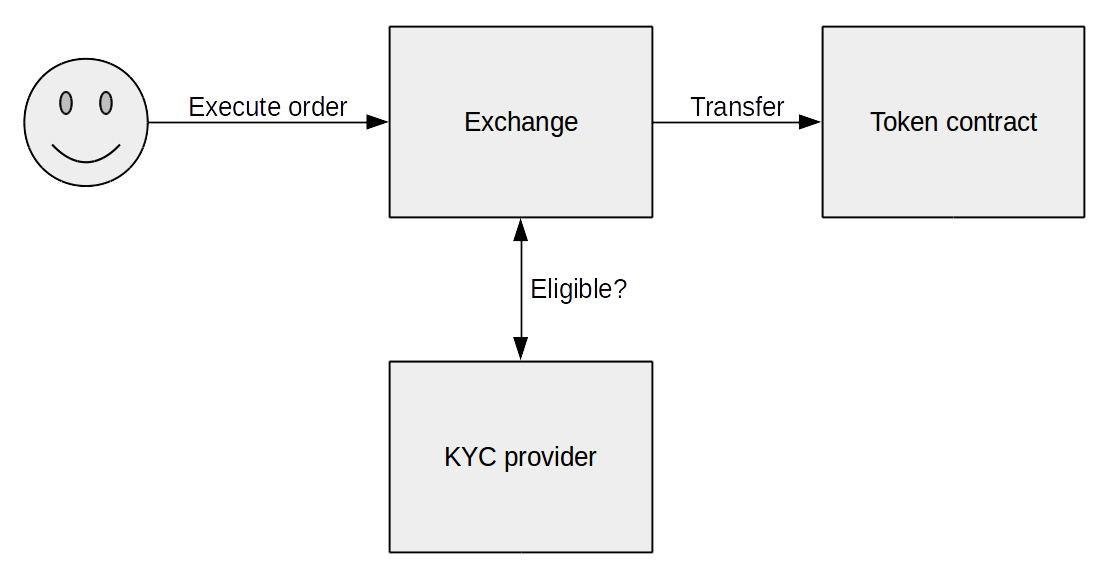
\includegraphics[width=0.8\textwidth]{figure-kyc-exchange}
	\caption{KYC-compliant exchange.}
	\label{fig:KYCCompliantExchange}
\end{figure}

Consider an established exchange that trades dozens of tokens.
It applies for official approval in a jurisdiction that requires all customers to pass the KYC procedure.
The governmental body acts as a KYC provider, deploys a KYC contract, and publishes its address.
The exchange adds KYC checks to its codebase and continues operation.
Users who do not want to apply for KYC can withdraw their tokens from the exchange.


\paragraph{KYC-compliant token}

If the token is KYC-compliant, the exchange does not need to be aware of the KYC (Figure~\ref{fig:KYCCompliantToken}).

\begin{figure}[h]
	\centering
	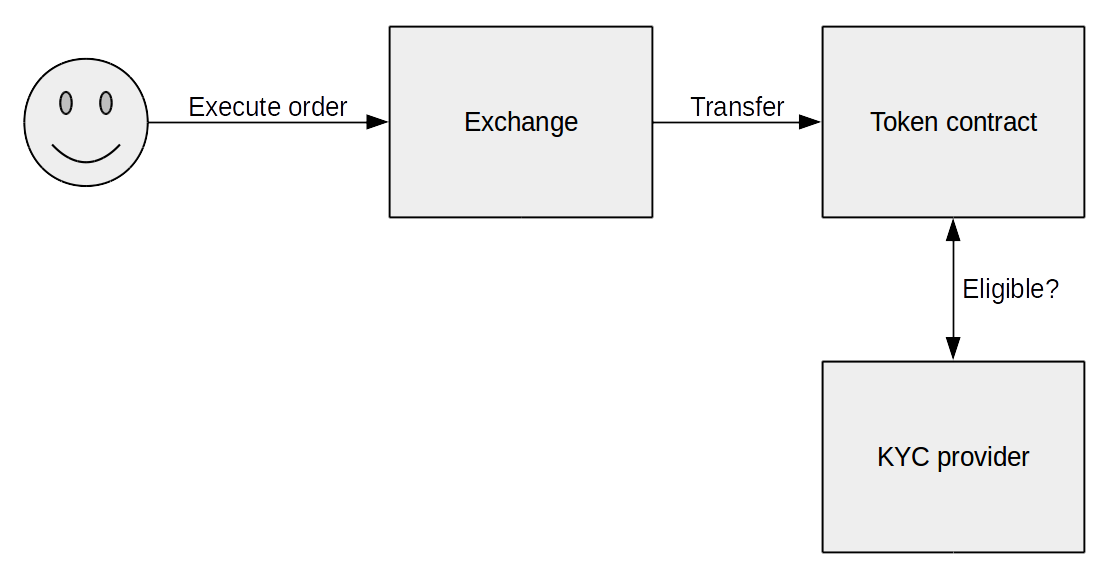
\includegraphics[width=0.8\textwidth]{figure-kyc-token}
	\caption{KYC-compliant token.}
	\label{fig:KYCCompliantToken}
\end{figure}

Consider a government that issues its own tokens.\footnote{Bank of England~\cite{Danezis2016} and the Monetary Authority of Singapore~\cite{Singapore17} have already researched this direction.}
KYC-approved users could use government tokens for tax payments, fees, and fines.
Such a solution leverages smart contracts' flexibility and auditability while only allowing approved entities to use the token.
The KYC-enabled government token can also be traded on exchanges, which would allow citizens to hold currency portfolios of their choice and only purchase government tokens to transact with the state.

\paragraph{Transaction-dependent checks}

Many jurisdictions impose restrictions that depend on the value of the transaction.
E.g.,~the EU regulation~\cite{EU847} states that "the obligation to check whether information on the payer or the payee is accurate should \textelp{} be imposed only in respect of individual transfers of funds that exceed \EUR{1\,000}".
EU member states impose further restrictions for large transactions, e.g.,~exceeding \EUR{10\,000} in Belgium, \EUR{15\,000} in Germany and in the Netherlands~\cite{PWC2015}.
Either the exchange contract or the token contract can perform such checks by storing the following mappings:
\begin{itemize}
	\item address $=>$ accumulated transaction volume in the current period (day, month, year);
	\item address $=>$ timestamp of the latest transaction. 
\end{itemize}


\section{Implementation details}

We created an initial (not privacy-preserving) implementation of the proposed design.
Our project consists of two smart contracts written in Solidity: KycProvider and KyceToken.
KycProvider maintains a 2-dimensional boolean array that stores the eligibility status across users and tokens.
On initialization, the address that deploys the contract is appointed as the \textit{owner}, allowing it to add and remove users from the whitelist.
The ownership may be transferred (using the functionality inherited from the standard \texttt{Ownable} contract).

The KycProvider exposes the following API:

\begin{itemize}
	\item \texttt{add(address \_user, address \_token)} makes the user eligible for using the token (callable only by the owner);
	\item \texttt{remove(address \_user, address \_token)} makes the user not eligible for using the token (callable only by the owner);
	\item \texttt{isEligible(address \_user, address \_token)} checks if the user is eligible for using the token.
\end{itemize}

KyceToken adheres to the de-facto standard token API in Ethereum -- ERC20.
To minimize the risk of security issues due to implementation subtleties, we inherit a widely used and tested ERC20 implementation by OpenZeppelin.
We override the functions \texttt{approve}, \texttt{transfer}, and \texttt{transferFrom} to check if the given user (\texttt{msg.sender}) is eligible for using this token.
If \texttt{isEligible} returns \texttt{false}, the execution stops.
If it returns \texttt{true}, the corresponding function of the superclass is invoked.

The implementation of the proposed scheme requires certain cryptographic primitives.
Some of them are already partially available in Ethereum as pre-compiled contracts (namely, elliptic curve addition, scalar multiplication, and pairing checks).
For the proposed scheme to be fully implemented, pairing evaluation is also required.\footnote{As of 2020, Ethereum does not support pairing evaluation.}


\section{Related work}

Jos{\'{e}} Parra Moyano and Omri Ross use distributed ledgers to improve the KYC process~\cite{Moyano2017}.
Their proposal can be summarized as follows:
\begin{itemize}
	\item the regulator maintains a database with all users' private data;
	\item the users signs a contract with their first bank (the\textit{home bank});
	\item the home bank stores hashes of the user's documents in a smart contract in a permissioned blockchain;
	\item when a user signs a contract with another bank it obtains the user's documents from the database and looks up the hash to ensure that the user has been KYC-approved;
	\item the identity of the home bank is not revealed;
	\item a cost-sharing mechanism for banks allows to proportionally share the cost of the initial KYC approval.
\end{itemize}
In this design, all banks store users' private data -- contrary to our solution, where it is stored only with the KYC provider.
The authors also propose a more decentralized design but claim it to be of lesser practical relevance.

Clare Sullivan and Eric Burger investigate possible implications of further development of the Estonian e-residency program using blockchain technology~\cite{Sullivan2017}.
E-residency of Estonia is a governmental program that provides applicants with a digital identity that can be used, e.g.,~to register a company and open a bank account.
Estonian e-residency disconnects a digital identity from citizenship or physical residence.
Within the e-residency program, Estonia collaborates with a blockchain project Bitnation~\cite{Bitnation15, Estonia15}.
Provable (previously known as Oraclize) implemented a connector that lets Ethereum contracts handle e-residency identities~\cite{Provable}.

A project~\cite{Ohtamaa2016} similar to ours implements a KYC scheme using Ethereum, but stores the KYC status on-chain in plaintext.
Multiple projects aim at easing customer onboarding for banks~\cite{CambridgeBlockchain, KycChain, SnapSwap, Tradle}.
Blockchain consortium R3 developed a proof-of-concept implementation of a shared KYC between ten banks based on its blockchain platform Corda~\cite{Allison2016}.
Multiple Ethereum-based identity projects have been proposed~\cite{Mesropyan2017, Sovrin, Uport}.


\section{Conclusion}

We have proposed a modular design of an Ethereum-based financial service with an external KYC check, which benefits all participants.

\begin{itemize}
	\item \textbf{Users} obtain a unified identity that they can use with multiple financial services.
	Users' data is stored only with the KYC provider and can be easily updated.
	Personal data is neither stored on the blockchain nor transmitted to third parties.
	\item \textbf{Financial services} greatly simplify the KYC process: it boils down to a single API call.
	Our design lets them cut KYC costs while at the same time diminishing risks of handling sensitive data.
	\item \textbf{Governments} get an opportunity to stimulate innovation in the financial sector by providing a unified and simple KYC API, which is especially relevant in rapidly growing fintech and blockchain industries.
\end{itemize}

Our design is agnostic to the nature of the entity behind the KYC contract.
It does not have to be a government body.
The proposed solution can be used in any setting where a smart contract based service wants to limit the set of its users.
For instance, many jurisdictions (e.g.,~the~US~\cite{SEC}) only allow certain investments to be offered to "accredited investors."
These are typically high-net-worth individuals and financial institutions.
This logic can be replicated in a blockchain setting.
Consider a blockchain-based financial service that only accepts cryptocurrency users who possess more than $10\,000$~USD and have done their first transaction before~2017.
The "accrediting" functionality is delegated to a third party KYC provider.
Proving net worth and previous activity on the blockchain is straightforward.
More checks can be added.
Once accredited, an investor can use multiple "restricted" services without revealing any personal details to their developers.
